\documentclass[12pt,oneside]{udthesis}\usepackage[]{graphicx}\usepackage[]{color}
% maxwidth is the original width if it is less than linewidth
% otherwise use linewidth (to make sure the graphics do not exceed the margin)
\makeatletter
\def\maxwidth{ %
  \ifdim\Gin@nat@width>\linewidth
    \linewidth
  \else
    \Gin@nat@width
  \fi
}
\makeatother

\definecolor{fgcolor}{rgb}{0.345, 0.345, 0.345}
\newcommand{\hlnum}[1]{\textcolor[rgb]{0.686,0.059,0.569}{#1}}%
\newcommand{\hlstr}[1]{\textcolor[rgb]{0.192,0.494,0.8}{#1}}%
\newcommand{\hlcom}[1]{\textcolor[rgb]{0.678,0.584,0.686}{\textit{#1}}}%
\newcommand{\hlopt}[1]{\textcolor[rgb]{0,0,0}{#1}}%
\newcommand{\hlstd}[1]{\textcolor[rgb]{0.345,0.345,0.345}{#1}}%
\newcommand{\hlkwa}[1]{\textcolor[rgb]{0.161,0.373,0.58}{\textbf{#1}}}%
\newcommand{\hlkwb}[1]{\textcolor[rgb]{0.69,0.353,0.396}{#1}}%
\newcommand{\hlkwc}[1]{\textcolor[rgb]{0.333,0.667,0.333}{#1}}%
\newcommand{\hlkwd}[1]{\textcolor[rgb]{0.737,0.353,0.396}{\textbf{#1}}}%
\let\hlipl\hlkwb

\usepackage{framed}
\makeatletter
\newenvironment{kframe}{%
 \def\at@end@of@kframe{}%
 \ifinner\ifhmode%
  \def\at@end@of@kframe{\end{minipage}}%
  \begin{minipage}{\columnwidth}%
 \fi\fi%
 \def\FrameCommand##1{\hskip\@totalleftmargin \hskip-\fboxsep
 \colorbox{shadecolor}{##1}\hskip-\fboxsep
     % There is no \\@totalrightmargin, so:
     \hskip-\linewidth \hskip-\@totalleftmargin \hskip\columnwidth}%
 \MakeFramed {\advance\hsize-\width
   \@totalleftmargin\z@ \linewidth\hsize
   \@setminipage}}%
 {\par\unskip\endMakeFramed%
 \at@end@of@kframe}
\makeatother

\definecolor{shadecolor}{rgb}{.97, .97, .97}
\definecolor{messagecolor}{rgb}{0, 0, 0}
\definecolor{warningcolor}{rgb}{1, 0, 1}
\definecolor{errorcolor}{rgb}{1, 0, 0}
\newenvironment{knitrout}{}{} % an empty environment to be redefined in TeX

\usepackage{alltt}

%----------------------------------------------------------------------------------------
%	Atributes Settings
%----------------------------------------------------------------------------------------
% About your study degree programme
\def \study{ITM} % possible options: ITM, SWD, MSD, IRM, IMS

% More about you and your thesis:
\def \Title{TESIS}
\def \title{PRA TESIS}
\def \subtitle{Preferensi Pengunjung Waterfront di Kota Parepare Sebagai Kota Wisata}
\def \yourName{Muhammad Uliah Shafar}
\def \yourIdentifier{21020119420029}
\def \yourPlace{<place>}
\def \submissionDate{<date>}  % month year. e.g. June 2017
\DTMsavedate{tanggalberita}{2021-01-31} %tanggal sidang
\def \hariBerita{<day>} %hari sidang
\def \yourAdvisor{Dr. Ars. Ir. Wijayanti, M.Eng}
\DTMsavetime{waktuberita}{24:60:60} %waktu sidang
\def \yourNipAdvisor{196307111990012001}
\def \yourSecAdvisor{Prof. Dr. Ir. Atik Suprapti,  M.T.}
\def \yourNipSecAdvisor{196511131998032001}
%\def \thisDocumentIsA{Thesis} % possible options:
                     % Thesis  .... for Master's Thesis   / Masterarbeit
                     % Thesis  .... for Bachelor's Thesis / Bachelorarbeit
                     % Seminar .... for Seminar Work      / Seminararbeit
                     % Project .... for Project Work      / Projektarbeit

% ITM/SWD/IRM: you could possibly write in German.
%\def \yourLanguage{english} % possible options: german, english
\IfFileExists{upquote.sty}{\usepackage{upquote}}{}
\begin{document}


% Child with Latex code only:


%--------------------------------------------------------------------------------------
% R chunk
%--------------------------------------------------------------------------------------

%--------------------------------------------------------------------------------------

\begin{titlepage}
	\begin{center}

\mbox{}\vfill

  {\bf \Title \par}

    \vspace{2\baselineskip}
		
\includegraphics[width=0.20\textwidth]{figures/logo}

    \vspace{2\baselineskip}

		{\large\bf\MakeUppercase \subtitle}

    \vspace{\baselineskip}
    Disusun dalam rangka memenuhi persyaratan\\ Program Studi Magister Arsitektur\\
    \vspace{\baselineskip}
        {\bf
           {\MakeUppercase\yourName}\\
           \yourIdentifier
        }

    \vspace{3\baselineskip}
		{\large\bf PROGRAM STUDI MAGISTER ARSITEKTUR DEPARTEMEN ARSITEKTUR FAKULTAS TEKNIK\\ UNIVERSITAS DIPONEGORO\\
			SEMARANG\\
			2021
		}
	\end{center}
\vfill\mbox{}

\end{titlepage}

\begin{titlepage}
	\begin{center}

\mbox{}\vfill

  {\bf \title \par}

    \vspace{3\baselineskip}
		
\includegraphics[width=0.20\textwidth]{figures/logo}

    \vspace{3\baselineskip}

		{\large\bf\MakeUppercase \subtitle}

    \vspace{3\baselineskip}
    disusun oleh\\
        {\bf
           {\MakeUppercase\yourName}\\
           \yourIdentifier
        }

    \vspace{3\baselineskip}
		{\large\bf PROGRAM STUDI MAGISTER ARSITEKTUR DEPARTEMEN ARSITEKTUR FAKULTAS TEKNIK\\ UNIVERSITAS DIPONEGORO\\
			SEMARANG\\
			2021
		}
	\end{center}
\vfill\mbox{}

\end{titlepage}

\pagenumbering{roman}
\chapter*{HALAMAN PERNYATAAN ORIGINALITAS}
\addcontentsline{toc}{chapter}{HALAMAN PERNYATAAN}
\begin{center}
 Dengan ini saya sebagai penulis menyatakan bahwa Pra Tesis dengan judul \subtitle\,adalah hasil karya saya sendiri. Semua data yang dicantumkan dan sumber referensi yang dikutip pada Pra Tesis ini adalah benar dan dapat dipertanggungjawabkan keasliannya.
\end{center}

\vspace{8\baselineskip}

\begin{flushright}
\begin{tabular}{@{}l}

Semarang, \DTMtoday \\
Penulis, \\
\\
\\
\\
\underline{Muhammad Uliah Shafar} \\
NIM. 21020119420029

\end{tabular}

\end{flushright}
\clearpage

% Validation -------------------------------------------------------------------------
\chapter*{\large\MakeUppercase\subtitle}
\addcontentsline{toc}{chapter}{HALAMAN PENGESAHAN}
\begin{center}
   Oleh :\\
   {\MakeUppercase \yourName}\\
   \yourIdentifier

\vspace{2\baselineskip}
{\small Diajukan pada Sidang Pra Tesis\\ Pada tanggal \DTMtoday}


\vspace{3\baselineskip}
Semarang, \DTMtoday

\vspace{2\baselineskip}

\begin{tabular}{@{}ccc@{}}
Pembimbing I	 & & Pembimbing II\\
	 & & \\
	 & & \\
	 & & \\
\yourAdvisor & & \yourSecAdvisor \\

\yourNipAdvisor & & \yourNipSecAdvisor \\
\end{tabular}

\vspace{2\baselineskip}

Mengetahui\\
Ketua Program Studi \\
Magister Arsitektur Departemen Arsitektur\\
Fakultas Teknik Universitas Diponegoro\\

\vspace{3\baselineskip}

Dr.Ir.Suzanna Ratih Sari, M.M., M.A.\\NIP. 196704301992032002
\end{center}

% Agreement -------------------------------------------------------------------------

\chapter*{HALAMAN PERNYATAAN PERSETUJUAN PUBLIKASI\\ TESIS UNTUK KEPENTINGAN AKADEMIS}
\addcontentsline{toc}{chapter}{HALAMAN PERNYATAAN PERSETUJUAN}

Sebagai sivitas academia Universitas Diponegoro, saya yang bertandatangan dibawah ini:

\begin{tabular}{@{}l@{\hspace{1em}:}@{\hspace{1em}}p{.65\textwidth}}
    Nama &  \yourName \\
    NIM & \yourIdentifier \\
    Program Studi & Magister Arsitektur \\
    Departemen & Arsitektur \\
    Fakultas & Teknik \\
    Jenis Karya & Tesis \\
\end{tabular}

Demi pengembangan ilmu pengetahuan, menyetujui untuk memberikan Hak Bebas Royalti Nonekslusif (None-Exclusive Royalty Free Right) atas karya ilmiah saya yang berjudul \subtitle.

Dengan hak tersebut, Universitas Diponegoro berhak menyimpan,\\ mengalihmedia/ formatkan, mengelola dalam bentuk pangkalan data (database),merawat dan mempublikasikan tugas akhir saya selama tetap mencantumkan nama saya sebagai penulis/pencipta dan sebagai pemilik Hak Cipta.

Demikian pernyataan ini saya buat dengan sebenar-benarnya.
\vspace{2\baselineskip}
\begin{flushright}
\begin{tabular}{@{}l@{\hspace{1em}:}l}
Dibuat di & Semarang\\
Pada tanggal & \DTMtoday\\
\end{tabular}

\vspace{2\baselineskip}
\begin{tabular}{@{}l}

Yang Menyatakan
\\
\\
\\
\yourName \\
\end{tabular}
\end{flushright}
\clearpage

% Prakata -------------------------------------------------------------------------
\chapter*{\ttfamily\large PRAKATA}
\addcontentsline{toc}{chapter}{PRAKATA}

\begin{prakata}

\lipsum[1-1]
\end{prakata}

% Abstrak -------------------------------------------------------------------------
\begin{abstract}
\addcontentsline{toc}{chapter}{ABSTRAK}
    Your text here\ldots
Write the abstract in English and in German, called \emph{Zusammenfassung}.
Describe in about 250 to 350 words the problem, the innovation, the method, the results and implications.

\end{abstract}

\noindent Kata kunci: lorem, ipsum, lorem, ipsum

% Abstract -------------------------------------------------------------------------
\chapter*{ABSTRACT}
\addcontentsline{toc}{chapter}{ABSTRACT}

Your text here Write the abstract in English and in German, called \emph{Zusammenfassung}.
Describe in about 250 to 350 words the problem, the innovation, the method, the results and implications.

\vspace{\baselineskip}
\noindent Keywords: lorem, ipsum, lorem, ipsum

% Acknogledge -------------------------------------------------------------------------
\chapter*{KATA PENGANTAR}
\addcontentsline{toc}{chapter}{KATA PENGANTAR}

Thanks to \ldots \lipsum[2-2]

\vspace{2\baselineskip}
\begin{flushright}
\begin{tabular}{@{}l}

Semarang, \DTMtoday \\
\\
\\
\yourName \\
\end{tabular}
\end{flushright}
\clearpage

%----------------------------------------------------------------------------------------
% TOC
%\tableofcontents
%\clearpage
%\addcontentsline{toc}{chapter}{\listfigurename}
%\listoffigures
%\clearpage
%\addcontentsline{toc}{chapter}{\listtablename}
%\listoftables

\clearpage
\pagenumbering{arabic}

% Child with Latex code only:


%--------------------------------------------------------------------------------------
% R chunk
%--------------------------------------------------------------------------------------
% Set parent


% load stat

%------------------------------------------------------

%------------------------------------------------------



\newcommand{\pieChartFig}
{\begin{figure}[h]
\centering

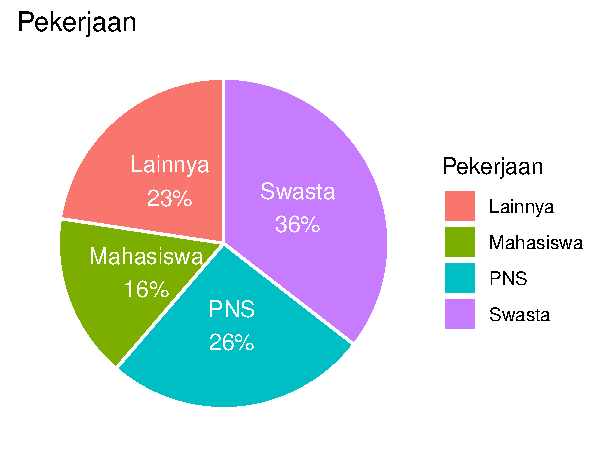
\includegraphics[width=\maxwidth]{../figures/stats2-1} 
\caption{Pie Chart Pekerjaan}
\label{pieChartFig}\end{figure}
}



\newcommand{\tabRegresi}{
% latex table generated in R 4.0.3 by xtable 1.8-4 package
% Fri Mar 19 20:38:25 2021
\begin{table}[ht]
\centering
\begin{tabular}{lrrrrr}
  \hline
 & Df & Sum Sq & Mean Sq & F value & Pr($>$F) \\ 
  \hline
data2\$total\_fit & 1.000 & 96.998 & 96.998 & 3.679 & 0.065 \\ 
  Residuals & 29.000 & 764.551 & 26.364 &  &  \\ 
   \hline
\end{tabular}
\caption{Regresi Linear} 
\label{tabRegresi}
\end{table}
}

%--------------------------------------------------------------------------------------


\chapter{Pendahuluan}\label{chap:pendahuluan}

\section{Latar Belakang}
\cite{imansari2015}
\lipsum[2-4]

\section{Rumusan Masalah}
\lipsum[2-4]

\begin{enumerate}
    \item  Lorem Ipsum ?
    \item Lorem Ipsum ?
\end{enumerate}


\section{Tujuan Penelitian}
\lipsum[2-4]
\section{Manfaat Penelitian}

\lipsum[2-4]
\begin{enumerate}
\item Lorem Ipsum
\item Lorem Ipsum
\end{enumerate}


\section{Sistematika Penulisan}
\lipsum[1-1]
\begin{itemize}
	\item Bab 1 : Pendahuluan\\
Bab terdiri dari latar belakang permasalahan, perumusan masalah, tujuan penelitian, manfaat penelitian, dan sistematika penulisan.
	\item Bab 2 : Tinjauan Pustaka\\
Bab ini terdiri dari landasan teori yang digunakan untuk memperkuat penemuan masalah, penelitian terdahulu dan kerangka pemikiran.
	\item Bab 3 : Metodologi Penelitian\\
Bab ini terdiri dari penjelasan variabel dan jenis paradigma yang digunakan untuk mencapai penemuan sesuai rumusan masalah, populasi, sampel, dan cara pengumpulan data.
	\item Bab 4 : Hasil dan Pembahasan\\
Bab ini terdiri dari pembahasan mengenai hasil - hasil penelitian yang berupa data-data yang didapatkan, dengan melakukan pengolahan terhadap indikator-indikator kenyamanan. Setelah pengelolahan bahan-bahan tersebut, analisis diperlukan untuk menemukan penemuan penelitian. Analisis diarahkan untuk menjawab rumusan masalah.
	\item Bab V : Kesimpulan\\
Bab terakhir terdiri dari kesimpulan yang didapatkan dari analisis terhadap permasalahan yang terdapat pada penelitian ini, sehingga penemuan bersama saran-saran dari penelusi dapat menghasilkan apa yang diinginkan.


\end{itemize}
\begin{comment}
\section{Alur Pikir}

\begin{figure}[hp]
\centering
\begin{tikzpicture}[node distance=2cm]
\node (ltr) [startstop] {Latar Belakang};

\node (rum) [startstop, right of=ltr, xshift=2cm] {Perumusan Masalah};

\node (tuj) [startstop, below of=rum, yshift=0.5cm] {Tujuan Penelitian};


\node (pus) [startstop, below of=tuj, yshift=0.5cm] {Studi Pustaka};


\node (kaj) [startstop, below of=pus, text width=3.5cm, xshift= -4cm, yshift=.5cm] {
	\textbf{Kajian Teori}\\ - Fitur binaan\\ - Aktivitas Luar
};


\node (kaj2) [startstop, below of=pus, text width=3.5cm, xshift= 4cm, yshift=.5cm] {
	\textbf{Gambaran Objek}\\ Fitur Binaan dan Aktivitas Luar Jl. Pinggir Laut
};


\node (hip) [startstop, below of=pus, yshift=-.5cm] {Hipotesa};


\node (met) [startstop, below of=hip, yshift=-.75cm, text width=7cm] {
	\textbf{Metode Peneltian}\\ Menggunakan Metode penelitian Kuantitatif Rasionalistik

	\textbf{Variabel}\\
	- Bebas : Fitur Binaan\\
	- Terikat : Aktivitas Luar\\

	\textbf{Sumber data}: Observasi dan Kuesioner
};

\node (ana) [startstop, below of=met, text width=8cm, yshift=-2cm] {
		\textbf{Analisis Data Statistik}\\ Penelitian ini menggunakan metode statika berupa uji regresi guna mengetahui pengaruh variabel fitur binaan terhadap variabel aktivitas luar.
};

\node (tem) [startstop, below of=ana, yshift=-.25cm] {Temuan Penelitian};

\node (kes) [startstop, below of=tem, yshift=.6cm] {Kesimpulan dan Rekomendasi};

\draw [arrow] (ltr) -- (rum);
\draw [arrow] (rum) -- (tuj);
\draw [arrow] (tuj) -- (pus);

\draw [arrow] (pus) -| (kaj);
\draw [arrow] (pus) -| (kaj2);

\draw [doublearrow] (kaj) -- (kaj2);

\draw [arrow] (kaj) |- (met);
\draw [dotted] (kaj) |- (hip);

\draw [arrow] (kaj2) |- (met);
\draw [dotted] (kaj2) |- (hip);

\draw [arrow] (met) -- (ana);
\draw [arrow] (ana) -- (tem);

\draw [arrow] (tem) -- (kes);

\end{tikzpicture}
\caption{Alur Pikir}
\end{figure}
\end{comment}
\newpage

\chapter{Tinjauan Pustaka}\label{chap:pstk}

\lipsum[2-4]

\section{Kerangka Penelitian}


Dari hasil tinjauan pustaka peneliti menyusun kerangka penelitian berdasarkan variabel-variable yang layak diteliti.


\begin{figure}[htbp]
\centering
\begin{tikzpicture}[node distance=2cm]

	\node (tit) [startstop, text width= 5cm] {Fitur Fisik Binaan pada Aktivitas Luar Jl. Pinggir Laut};

	\node (va1) [startstop, below of=tit, text width=5cm, xshift=-3cm] {Variabel Bebas\\ Fitur Fisik Binaan};

	\node (va2) [startstop, below of=tit, text width=5cm, xshift=3cm] {Variabel Tergantung\\ Aktivitas Luar};

	\node (de1) [startstop, below of=va1, text width=5cm, yshift=-2cm] {
		\textbf{Sub Variabel Bebas}\\
		- Elemen Jalan \\
		- Kualitas Jalan \\
		- Elemen Tempat Duduk \\
		- Kualitas Tempat Duduk \\
		- Elemen Alami \\
		- Kualitas Alami \\
		- Fasilitas \& Aminities \\
		- Estetika \\

	};
	\node (de2) [startstop, below of=va2, text width=5cm, yshift=-2cm] {
			\textbf{Sub Variable Tergantung}\\
		- Aktivitas relaxsasi\\
		- Aktivitas fisik\\
		- Travel aktif\\
		- Interaction with wildlife and nature\\
		- Interaksi sosial\\
		- Partisipasi di aktivitas grup\\
		};
\draw [arrow] (tit) -| (va1);
\draw [arrow] (va1) -- (de1);
\draw [arrow] (tit) -| (va2);
\draw [arrow] (va2) -- (de2);

\end{tikzpicture}
\caption{Alur Pikir}
\end{figure}

\chapter{Metodologi Penelitian}\label{chap:method}

\section{Metode dan Jenis Penelitian}

\lipsum[2-4]

\section{ Knitr child Documents}
You should note that using knitr package you can easily incorporate difference kinds of files into a project.

\tabRegresi
\pieChartFig

\chapter{Kesimpulan}\label{chap:kesimp}

% Child with Latex code only:


%--------------------------------------------------------------------------------------
% R chunk
%--------------------------------------------------------------------------------------

%--------------------------------------------------------------------------------------

\chapter*{BERITA ACARA SIDANG PRA TESIS}
\addcontentsline{toc}{chapter}{BERITA ACARA}
\setlength\parindent{0pt}
Dengan ini saya selaku peserta sidang menyatakan bahwa telah melaksanakan sidang Pra Tesis pada:


\begin{tabular}{@{}l@{\hspace{1em}:}@{\hspace{1em}}l@{}}
    Hari &  \hariBerita\\
    Tanggal & \DTMusedate{tanggalberita} \\
    Waktu & \DTMusetime{waktuberita}\\
    Tempat & \yourPlace\\
\end{tabular}

\vspace{\baselineskip}
{\bf Dilakukan oleh:}

\begin{tabular}{@{}l@{\hspace{1em}:}@{\hspace{1em}}p{.75\textwidth}}
    Nama &  \yourName \\
    NIM & \yourIdentifier \\
    Judul & \subtitle \\
\end{tabular}

\vspace{\baselineskip}
{\bf Dengan susunan tim penguji:}

\begin{tabular}{@{}l@{\hspace{1em}:}@{\hspace{1em}}l@{}}
    Pembimbing I & \yourAdvisor \\
    Pembimbing II & \yourSecAdvisor \\
\end{tabular}

\vspace{\baselineskip}
{\bf Pelaksanaan sidang:}
\begin{enumerate}[leftmargin = *]
    \item Sidang Pra tesis dengan judul \subtitle. Dimulai pada pukul \DTMusetime{waktuberita}.
\end{enumerate}

\vspace{\baselineskip}
{\bf Daftar Pertanyaan:}

{\bf \yourAdvisor}
\begin{enumerate}[leftmargin = *]
    \item \ldots
    \item \ldots
    \item \ldots
\end{enumerate}
\vspace{\baselineskip}
{\bf \yourSecAdvisor}
\begin{enumerate}[leftmargin = *]
    \item \ldots
    \item \ldots
    \item \ldots
\end{enumerate}

\vspace{\baselineskip}
Demikian berita acara sidang Pra Tesis ini dibuat sesuai dengan keadaan yang sebenar-benarnya. \ldots
\vspace{30pt}

\begin{flushright}
\begin{tabular}{@{}l}

Semarang, \DTMtoday \\
Peserta sidang,
\\
\\
\\
\\
\yourName \\
NIM.\yourIdentifier
\end{tabular}
\end{flushright}

\begin{center}
\vspace{\baselineskip}
Mengetahui

\begin{tabular}{@{}ccc@{}}
Pembimbing I	 & & Pembimbing II\\
	 & & \\
	 & & \\
	 & & \\
\yourAdvisor & & \yourSecAdvisor \\

NIM.\yourNipAdvisor & & NIM.\yourNipSecAdvisor \\
\end{tabular}
\end{center}



\chapter*{DATA DIRI PENULIS}
\addcontentsline{toc}{chapter}{DATA DIRI PENULIS}

\begin{wrapfigure}[7]{l}{3cm}
\centering
    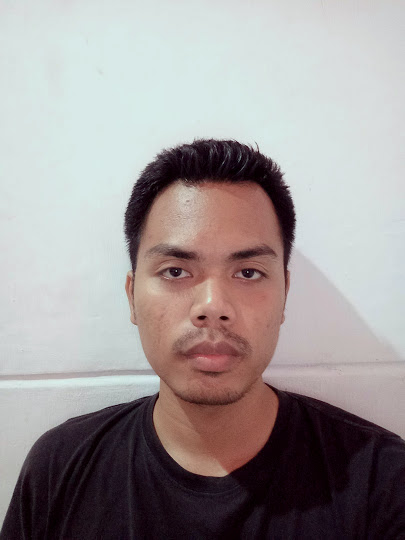
\includegraphics[width=2.8cm,trim=60 40 60 140,clip]{saya.jpg}
\end{wrapfigure}

\noindent Muhammad Uliah Shafar, pria kelahiran Parepare, 26 Juni 1996, sebagai putra sulung dari Parman Farid dan Junaeda. Lulus pendidikan S2 di Magister Arsitektur DAFT Undip, dengan alur konsentrasi Arsitektur Kota. Uliah menjalani pendidikan S2 sejak 2019 sesaat setelah menempuh pendididkan S1nya di UTY Yogyakarta.
Uliah mulai tertarik dengan bidang perkotaan sejak dia menonton film Spiderman sewaktu remaja. Ia melihat scene dimana spiderman berada di bawah jalan raya yang teknisnya disebut sistem pembuangan air kotor kota dan berpikir bahwa tempat tersebut tidak ada di kotanya dan mungkin itu memiliki kegunaan yang besar untuk seisi kota tersebut. Rasa keingintahuan terhadap bagaimana kota terbentuk menjadi latar belakang ia sangat bersemangat dalam menulis dan merancang hal-hal baru berkaitan sebuah kota yang terpelihara dan terorganisir dengan baik.

Saat ini tulisannya sudah ada yang terpublikasikan di jurnal nasional berkaitan dengan ruang publik. Ketekunannya dalam menulis membuatnya ingin merencanakan penulisan artikel-artikel di kemudian hari, bahkan dalam bahasa internasional. Uliah sangat tertarik dengan buku-buku perkotaan terutama dengan judul Making Place. Buku tersebut menurutnya sangat menarik karena dipadukan dengan ilmu sains dan seni praktis dalam menggambarkan realitas sebuah kota.

\vspace{2\baselineskip}
\begin{flushright}
    Hormat saya,\\ Muhammad Uliah Shafar
\end{flushright}

%----------------------------------------------------------------------------------------
%	BIBLIOGRAPHY
\bibliographystyle{apalike}
\bibliography{bibliography/biblio.bib}


\end{document}
